\begin{figure}[ht!]
    \begin{subfigure}{\textwidth}
    \centering
    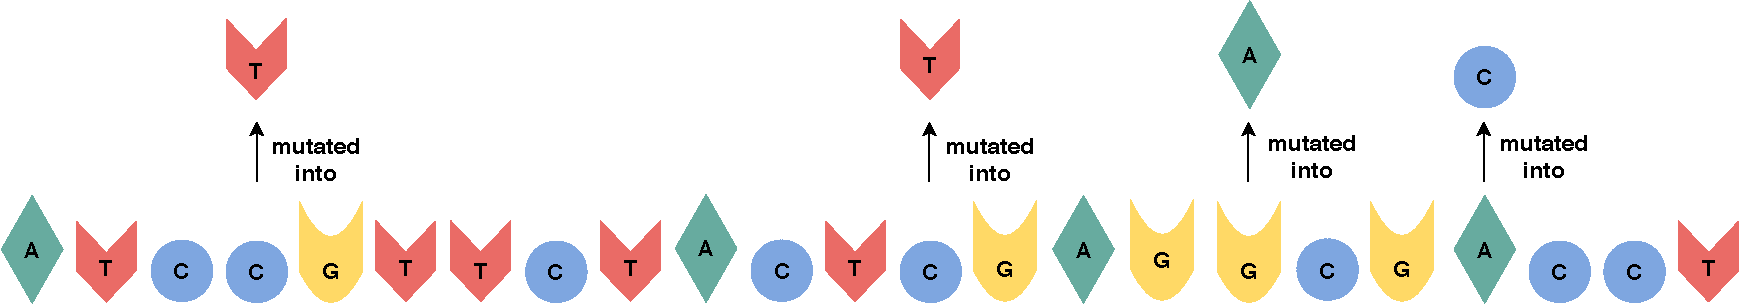
\includegraphics[scale=0.5]{graphics/sce_counts.pdf} \\
    \vspace{0.9cm}
    \begin{tabulary}{\columnwidth}{cc|cc|cc}
    \toprule
        \multicolumn{2}{c}{\textbf{1-mer}}  & \multicolumn{2}{c}{\textbf{3-mer}} & \multicolumn{2}{c}{\textbf{5-mer}} \\
        \hline
        mutation & count vector & mutation & count vector & mutation & count vector \\
    \hline
        [A$\rightarrow$C] & 1 & G[A$\rightarrow$C]C & 1 & CG[A$\rightarrow$C]CC & 1 \\
        
        [C$\rightarrow$T] & 2 & C[C$\rightarrow$T]G & 1 & TC[C$\rightarrow$T]GT & 1 \\
        
         &  & T[C$\rightarrow$T]G & 1 & CT[C$\rightarrow$T]GA & 1 \\
         
        [G$\rightarrow$A] & 1 & G[G$\rightarrow$A]C & 1 & AT[G$\rightarrow$A]CG & 1 \\
        
        ... & 0 & ... & 0 & ... & 0 \\
    \bottomrule
    \end{tabulary}
    \caption{Generating the count vector for 1-mer, 3-mer and 5-mer}\label{fig:get_sce}
    \end{subfigure} \\

  \vspace{1cm}
  \begin{subfigure}{\textwidth}
  \begin{minipage}{0.65\textwidth}
    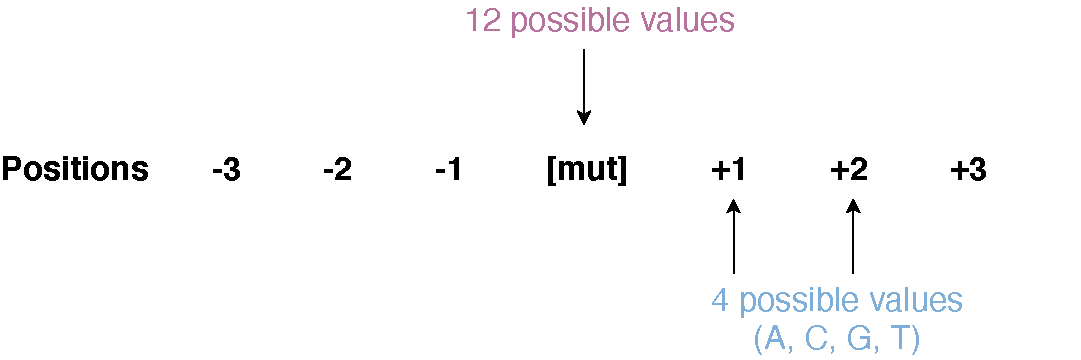
\includegraphics[width=\textwidth]{graphics/sce_counts_demo.pdf}
  \end{minipage}
  \begin{minipage}{0.3\textwidth}
    \begin{equation}
    l = 12 \times 4^{k-1}
    \label{eq:sce_counts}
    \end{equation}
    where $l$ is the number of elements and $k$ is the k-mer size, so $k-1$ is the number of flanking bases involved
  \end{minipage}
    \caption{Total number of elements for SCE incorporating flanking positions}\label{fig:sce_size}
  \end{subfigure} \\
  \vspace{0.2cm}
  \caption{
%   \textbf{The number of elements increases extremely rapidly with increasing k-mer size.} This is because there are 12 possible mutations, and for each flanking position, there are 4 possible bases. Panel (a) gives an example of how the count vector for SCE is generated for 1-mer, 3-mer and 5-mer for a DNA sequence with 4 mutations. The elements in the count vector were then divided by the total number of mutations to obtain the SCE vector. Panel (b) illustrates how to calculate the number of elements given the $k$-mer size. 
} \label{fig:sce_counts}
\end{figure}
